\chapter{INTRODUCCIÓN}



\section{SISTEMA DE PROCESAMIENTO DE LENGUAJE}
\begin{itemize}
    \item Subsistema dentro de una máquina que permite comunicar desde el exterior hasta el interior de la máquina
    \item No esta solo mediado por un lenguaje de programación. Este es solo una pieza del engranaje
    \item Generalmente son necesarios unos programas adicionales en el entrono computacional para que el compilador pueda tener un ejecutable y este se pueda ejecutar. Estos son:
    \begin{itemize}
        \item Preprocesador: Toma el programa fuente y detecta si hay elementos que se pueden obviar. Por ejemplo, librerías que ya estén previamente compiladas. Retorna un programa fuente modificado.
        \item Compilador: Toma el programa fuente modificado y lo traduce en un programa ensamblador. Este programa depende en gran medida de la máquina y del fabricante. Un traductor toma un programa fuente modificado y lo transforma en otro lenguaje preestablecido. Un compilador generalmente transforma un lenguaje de alto nivel a un lenguaje de bajo nivel. Por ejemplo de Java a C. Retorna el programa ensamblador
        \item Ensamblador: Toma el programa ensamblador y construye un código de maquina relocalizable. Es un código de maquina donde todo es lenguaje de maquina (es decir '0's y '1's) excepto las direcciones de memoria. Retorna el código de máquina relocalizable.
        \item Enlazador-cargador: Toma el código de máquina relocalizable. Resuelve las direcciones de memoria, y lo carga en memoria para que quede listo para ser ejecutado. Retorna un código de máquina destino
    \end{itemize}
    
   
\end{itemize}



\section{ESTRUCTURA DE UN COMPILADOR}

\begin{itemize}
    \item Analizador léxico: Toma el programa fuente y crea una secuencia de tokens. Remueve los comentarios, espacios en blanco, indentación innecesaria, etc. Esta compuesto por categorías léxicas. Estas definen el tipo de cada palabra. Ej: \\
    ``El jardín tiene flores''\\
    El analizador léxico encontraría primero la palabra ``El''. La clasificaría como un articulo, después con la palabra ``jardín'' la clasificaría como un sustantivo, etc. El resultado final seria similar a ``Articulo, sustantivo, verbo, sustantivo''. Eso es una secuencia de token. Retorna la secuencia de tokens.
    \item Analizador sintáctico: Toma la secuencia de tokens y verifica si esa secuencia de tokens se ajustan a un patrón para una gramática dada previamente definida. Crea un árbol sintáctico. Retorna el árbol sintáctico
    \item Analizador semántico: Toma el árbol sintáctico, realiza cambios sobre ese árbol que facilita la comprensión de la maquina y lo retorna como árbol semántico
    \item Generador de código intermedio: Toma el árbol semántico y realizando un proceso inverso al ya realizado genera un código intermedio y lo retorna.
    \item optimizador de código: Toma el código intermedio y reduce su tamaño o mejora el tiempo de ejecución de programa. Retorna un código intermedio optimizado
    \item Generador de código: Toma el código intermedio óptimo y lo transforma en código de la máquina de cada fabricante. Retorna el un código assembler para la maquina especificada
    \item Tabla se símbolos: Guarda información que no se debe perder a lo largo de la compilación o ejecución del programa. Es similar a una tabla de una base de datos.
    \item Módulo de manejo de errores: Facilita la detección de errores el el código fuente.
\end{itemize}


\section{TIPOS DE COMPILADORES}
\begin{itemize}
    \item De preprocesador: Limpian el código fuente
    \item Ensamblador: Toma el programa en assembler y lo pasa a código de maquina y resuelven las posiciones de memoria especificas.
    \item De carga y ejecución: Buscan la forma de llevar el programa desde el disco duro hasta la memoria
    \item De depuración: Se construyen para abordar el problema de como gestionar los errores que se presentan en todo el proceso de desarrollo de aplicaciones.
    \item De optimización: Toman el código intermedio y tratan de levar a un esquema mejor, que sea mas eficiente
    \item Metacompilador: LEX, YACC. Ayudan a crear analizadores léxicos o sintácticos de forma sencilla.
    \item De una pasada: Dependiendo de la complejidad del código fuente, solo es necesario leerlo completamente una vez para compilarlo.
    \item De múltiples pasadas:
    \item Compilador Cruzado: Se construyen en un entrono computación pero su ejecución es en otro entorno computacional (Ej: se compila en Linux, pero se usan para windows). Se usan para hacer productos en otras plataformas
    \item Autocompilador: Cuando el lenguaje de implementación es el mismo lenguaje de compilación
    \item Decompilador: Relacionado con la ingeniería inversa. Realizan el proceso inverso. Dado un lenguaje destino, cual fue el código fuente.
    
    
\end{itemize}


\section{INTERPRETES Y TRADUCTORES}
\begin{itemize}
 \item Un compilador toma un programa fuente y lo trasforma en un programa destino. El programa destino tomara sus datos de entrada y producirá datos de salida. En ese sentido el enfoque de un compilador es OFF-LINE.
\item Un interprete toma un programa fuente y unos datos de entrada y produce los datos de salida. Tiene un enfoque ON-LINE, es decir las instrucciones se ejecutan combinadas con los datos de entrada
\item Un compilador híbrido utiliza un traductor que toma un programa fuente para producir un programa en un lenguaje intermedio, que después ingresará a una máquina virtual junto con los datos de entrada para producir los datos de salida. Es un enfoque muy utilizado actualmente porque evita estar atados a la maquina del fabricante.
\end{itemize}
\section{ORGANIZACIONES COMPUTACIONALES}

\begin{figure}[H]
    \centering
    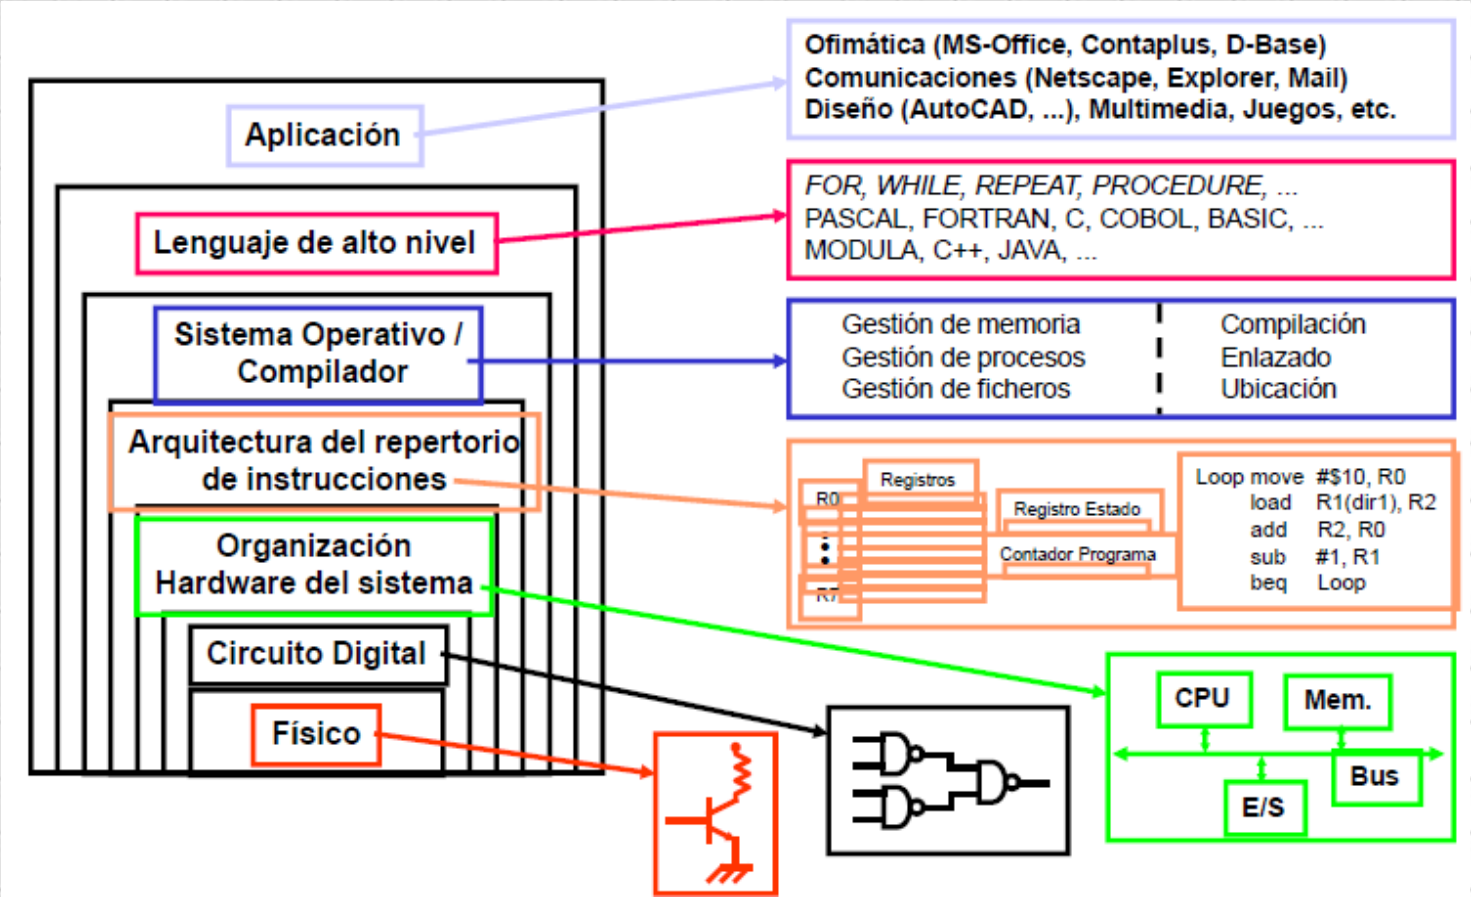
\includegraphics[width=0.8\textwidth, height=10cm,keepaspectratio]{chapters/chapter0/figures/Ubicacion lenguajes de programacion.png}
    \caption{Caption}
    \label{fig:my_label}
\end{figure}

\begin{itemize}
    \item El término ``organizaciones computacionales'' es personal. Generalmente se usa el término ``arquitecturas computacionales''. Sin embargo, se considera que el termino ``arquitecturas'' es demasiado rígido para hablar de computadores de naturaleza virtual
    \item Los lenguajes se pueden clasificar en generaciones:
    \begin{itemize}
        \item Primera generación: Lenguaje de nivel físico, donde el programador trabaja con los 0's y 1's de los circuitos digitales
        \item Segunda generación: Fortran, C, Cobol. De alto nivel
        \item Tercera generación: Lenguajes especializados en tareas especificas. Ej: R.
        \item: Cuarta generación: Lenguajes de programación mas abstractos con nuevos paradigmas de programación como OOP, etc.
        \item Quinta generación: Procesamiento simbólico, usados para Inteligencia artificial como Prolog.
    \end{itemize}
    
    \item Los lenguajes también se pueden clasificar en:
    \begin{itemize}
        \item Imperativos: Inspirado en la manera en la que los lenguajes naturales (Español, Ingles, Etc) donde la filosofía central esta en el verbo. La forma imperativa es de ordenes. Podría ser posible construir lenguajes de programación usando otras formas verbales donde los tiempos verbales o las hipótesis se podrían manejar.
        \item Declarativos: Trabajan en el como se deberían hacer las cosas. No trabajan con la parte física sino con la interpretación. No tienen estructuras de control como if, while, etc.
    \end{itemize}
    \item También pueden clasificarse dependiendo de su paradigma de programación.
    \item La capacidad expresiva de todas estas clasificaciones es igual, aunque la forma de solucionar un problema puede facilitarse dependiendo del tipo de lenguaje usado.
    \item Arquitectura computacional y lenguaje de programación van de la mano.
    
    \item Herramientas especializadas ara desarrollo de lenguajes de programación:
    \begin{itemize}
        \item Generadores de analizadores sintácticos: que producen automáticamente analizadores de sintaxis a partid de una descripción gramatical
        \item Generadores de analizadores léxicos: que producen analizadores léxicos a partid de la descripción de los tokens de un lenguaje mediante expresiones regulares
        \item Motores de traducción dirigidos por sintaxis: que producen colecciones de rutinas para recorrer un árbol de análisis y generar código intermedio
        \item: Generadores de generador de código: que producen un generador de código a partir de una colección de reglas para traducir cada operación del lenguaje intermedio al lenguaje de máquina para una máquina destino
        \item Motores de análisis de flujo de datos que facilitan la recopilación de información sombre como se transmiten los valores de una parte de un programa a la otra. El análisis del flujo de datos es una parte clave la optimización del código.
        \item Herramientas de contracción de un compilador: que proporcionan un conjunto integrado de rutinas para construir varias fases de un compilador
    \end{itemize}
    
\end{itemize}

\section{ROL DE LOS LENGUAJES DE PROGRAMACIÓN}
\section{EJERCICIOS DEL CAPÍTULO}
\begin{enumerate}
    \item Análisis, diseño e implementación de una máquina de Turing (MT), en el lenguaje de programación C#, que realice la división de dos números binarios de tres dígitos.
    
    \item Análisis, diseño e implementación de una máquina universal de Turing (MT), en el lenguaje de programación C#.
    
    \item Implementar ``El juego de la vida'' de Jhon Conway en el lenguaje de programación SWIFT.
    
    \item Demostrar que el modelo de Conway tiene computación universal.
\end{enumerate}